%%%%%%%%%%%%%%%%%%%%%%%%%%%%%%%%%%%%%%%%%
% Thin Sectioned Essay
% LaTeX Template
% Version 1.0 (3/8/13)
%
% This template has been downloaded from:
% http://www.LaTeXTemplates.com
%
% Original Author:
% Nicolas Diaz (nsdiaz@uc.cl) with extensive modifications by:
% Vel (vel@latextemplates.com)
%
% License:
% CC BY-NC-SA 3.0 (http://creativecommons.org/licenses/by-nc-sa/3.0/)
%
%%%%%%%%%%%%%%%%%%%%%%%%%%%%%%%%%%%%%%%%%

%----------------------------------------------------------------------------------------
%	PACKAGES AND OTHER DOCUMENT CONFIGURATIONS
%----------------------------------------------------------------------------------------

\documentclass[a4paper, 11pt]{article} % Font size (can be 10pt, 11pt or 12pt) and paper size (remove a4paper for US letter paper)
\usepackage{color}
\usepackage[protrusion=true,expansion=true]{microtype} % Better typography
\usepackage{graphicx} % Required for including pictures
\usepackage{wrapfig} % Allows in-line images
\usepackage{endnotes}
\usepackage{mathpazo} % Use the Palatino font
\usepackage[T1]{fontenc} % Required for accented characters
\linespread{1.05} % Change line spacing here, Palatino benefits from a slight increase by default
\usepackage{fancyhdr}
\usepackage[margin=1.25in]{geometry}
\pagestyle{fancy}
\fancyhf{}
\rhead{Reinforcement Learning Problem Set 21.06.2019}
\lhead{Adam, Freire, Serra, Wolf}
\rfoot{Page \thepage}
\usepackage{amsmath}
\usepackage{amssymb}
\usepackage{version}
\usepackage{setspace}
\usepackage{enumerate}
\usepackage{multicol}
\usepackage{amsfonts}
\usepackage{amssymb}
\usepackage{subcaption,graphicx}
\usepackage{rotating}
\usepackage{lscape}
\usepackage{pdflscape}
\usepackage{array,tabularx,float,dcolumn,lscape}
\usepackage{booktabs}
\usepackage{xr}
\usepackage{dcolumn}
\usepackage{hyperref}
\usepackage{amsmath}
\usepackage{algorithm}
\usepackage{tikz}
\usepackage[noend]{algpseudocode}
\graphicspath{ {../img/} }
\tikzset{every picture/.style={line width=0.75pt}} %set default line width to 0.75pt


\makeatletter
\def\BState{\State\hskip-\ALG@thistlm}
\makeatother

\newlength\tindent
\setlength{\tindent}{\parindent}
\setlength{\parindent}{0pt}
\renewcommand{\indent}{\hspace*{\tindent}}
\renewcommand{\familydefault}{\sfdefault}

\makeatletter
\renewcommand\@biblabel[1]{\textbf{#1.}} % Change the square brackets for each bibliography item from '[1]' to '1.'
\renewcommand{\@listI}{\itemsep=0pt} % Reduce the space between items in the itemize and enumerate environments and the bibliography

\renewcommand{\maketitle}{ % Customize the title - do not edit title and author name here, see the TITLE block below
\begin{flushright} % Right align
{\LARGE\@title} % Increase the font size of the title

\vspace{50pt} % Some vertical space between the title and author name

{\large\@author} % Author name
\\\@date % Date

\vspace{40pt} % Some vertical space between the author block and abstract
\end{flushright}
}

\begin{document}

\section*{Question 1}

Let $\phi : X x A \rightarrow \mathbb{R}^{d}$

The task is to compute $\nabla_{\theta}log(\pi_{\theta}(a|x))$ for the Boltzmann policy:
\begin{equation}
\pi_{\theta}(a | x)= \frac{e^{\theta^{\top} \phi(x, a)}}{\sum_{b} e^{\theta^{\top} \phi(x, b)}}
\end{equation}

To answer this, we take logs and the derivative:
\begin{align}
\nabla_{\theta} \log \pi_{\theta}(a | x)
&=\nabla_{\theta} \log \frac{e^{\theta^{\top} \phi(x, a)}}{\sum_{b} e^{\theta^{\top} \phi(x, b)}}  \\
&=\nabla_{\theta} \log e^{\theta^{\top} \phi(x, a)}-\nabla_{\theta} \log \sum_{b} e^{\theta^{\top} \phi(x, b)} \\
&=\phi(x, a)-\frac{1}{\sum_{b} e^{\theta^{\top} \phi(x, b)}}\sum_{b'} e^{\theta^{\top} \phi(x, b')} \phi(x, b') \\
& =\phi(x, a)-\sum_{b'} \frac{e^{\theta^{\top} \phi(x, b')} }{\sum_{b} e^{\theta^{\top} \phi (x, b)} } \phi(x, b')
\end{align}

Finally obtaining:
\begin{equation}
\nabla_{\theta}log(\pi_{\theta}(a|x)) = \phi(x, a)-\sum_{b} \pi_{\theta}(b|x) \phi(x, b)
\end{equation}

Which can be rewritten as:
\begin{equation}
\nabla_{\theta} \log \pi_{\theta}(a| x)=\phi(x, a)-\mathbb{E}_{\pi_{\theta}}[\phi(x, \cdot)]
\end{equation}


\section*{Question 2}
For this question, we built a policy gradient algorithm with a Boltzmann policy using $\phi_i(x,a) = 1_{(a=1)}$. In this section, we introduce the algorithm. We then answer the questions posed in the excercise in the following sections. \\

The MDP we study has one state $x$ (that is, $X=\{x\}$) and two actions $\mathcal{A}=\left\{a_{1}, a_{2}\right\}$. The rewards are defined as follows:

$$
R_{k}=\left\{\begin{array}{ll}{1,} & {\text { with probability } p_{I_{k}}} \\ {0,} & {\text { otherwise }}\end{array}\right.
$$

The rewards are received with probability $p_{1}=1 / 2$ and $p_{2}=1 / 2+\Delta$. Given the environment set-up, we define a learning algorithm in order to find the optimal policy $\pi_{\theta_{k}}$. We use the policy gradient method to learn the optimal weight parameters $\theta_{k+1}=\theta_{k}+\alpha_{k} g_{k}$. The arguments our algorithm takes are:

\begin{enumerate}
	\item Enviroment: Takes delta as argument and react to actions paying 1 or 0 with probability $p_{1}=1 / 2$ and $p_{2}=1 / 2+\Delta$.
	\item Gamma: Discount factor for future rewards.
	\item Policy: In this case we used Boltzmann policy as defined previously
	\item Seed: We choose a random seed to make sure it is possible to reproduce the simulations.
	\item Step type: Here we defined a fixed learning rate and also different rate decay in function of the number of steps.
	\item Delta: The environment parameter that gives how much the reward from action 2 is better than action 1.
	\item Weights $\theta$: Weights of our policy
	\item Beta: Learning rate for the value function
\end{enumerate}

The following plots show some training results obtained by averaging over various training runs, using different random states to initialize.

   \begin{figure}[!htb]
        \center{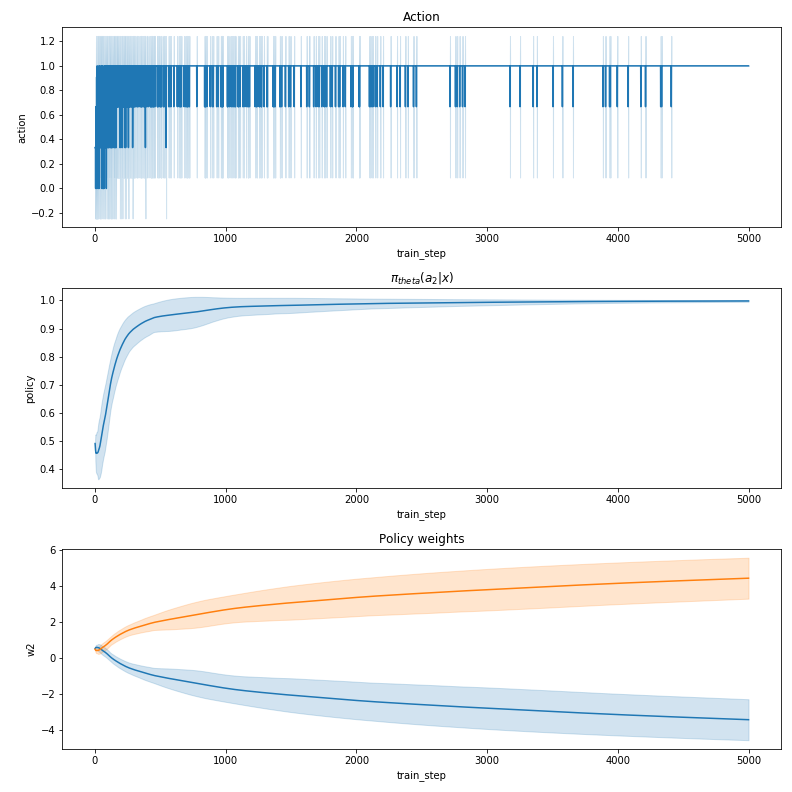
\includegraphics[width=\textwidth]
        {../img/policy_gradient_convergence.png}}
        \caption{\label{fig:my-label} Convergence of the algorithm}
      \end{figure}

The first plot shows the mean of actions taken over the training steps and the corresponding standard deviation. The second plot shows the convergence of the policy function and the third shows the evolution of the weights $\theta$. \\

Note that the policy values are plotted together with the standard deviation over different seeds. Policy function values cannot be higher than 1 or lower than 0, however, mean +- sd can be higher than 1. The main objective is to illustrate the volatility of the measure.

Having introduced the algorithm we built, we now move to answer the questions for the exercise.

\subsection*{Question 2.1}

Task: What is the influence of $\gamma$ on the algorithm.
\\
\\
\textbf{We find that $\gamma$ does not play a role in this policy gradient.} We get this result because we use the particularly simple estimation of the expectation in the policy gradient function suggested in the hint. When we set $h(x)=\gamma V^{\pi_{\theta_{k}}}(x)$, take a single sample to approximate the expectation, and take $\widehat{Q}^{\pi_{\theta_{k}}}\left(x, A_{k}\right)=R_{k}+\gamma V^{\pi_{\theta_{k}}}(x)$ , the expression for the policy gradient simplifies as follows:

\begin{align} \nabla_{\theta} \rho(\theta)
&=\sum_{(x, a) \in \mathcal{X} \times \mathcal{A}} \mu_{\theta}(x) \pi_{\theta}(a | x) \nabla_{\theta} \log \pi_{\theta}(a | x)\left(Q^{\pi_\theta}(x, a)-h(x)\right) \\
&=\mathbb{E}_{X \sim \mu_{\theta}, A \sim \pi_{\theta}(\cdot | X)}\left[\nabla_{\theta} \log \pi_{\theta}(A | X)\left(Q^{\pi_{\theta}}(X, A)-h(X)\right)\right] \\
&\approx \nabla_{\theta} \log \pi_{\theta}(a | x)  \left(\widehat{Q^{\pi_{\theta}}(x, a)}-h(x)\right) \\
&=\nabla_{\theta} \log \pi_{\theta}(a | x)  \left(R_{k}+\gamma V^{\pi_{\theta_{k}}}(x) - \gamma V^{\pi_{\theta_{k}}}(x)\right) \\
&=\nabla_{\theta} \log \pi_{\theta}(a | x)  R_{k} \\
&=\left(  \phi(x, a)-\sum_{b} \pi_{\theta}(b|x) \phi(x, b)\right)R_{k}
\end{align}

\textbf{The discount factor $\gamma$ cancels out.} Further, since the state in this MDP does not change, we do not have to take into account the consequences of our actions now for our future as we adjust our policy. Therefore the choice of  $\gamma$ should intuitively not play a role in our policy gradient.

\subsection*{Question 2.2}

Task: Fix $\gamma = 0.99$ and $\delta = 0.05$, and consider the step sizes $\frac{\alpha_{k}}{\sqrt{k}} ,\frac{\alpha_{k}}{k}, \text { and },\frac{\alpha_{k}}{k^{2}}$ for various choices of $c$. Plot $\pi_{\theta_{k}}(a_{2}|x)$ as a function of $k$. \\

   \begin{figure}[!htb]
        \center{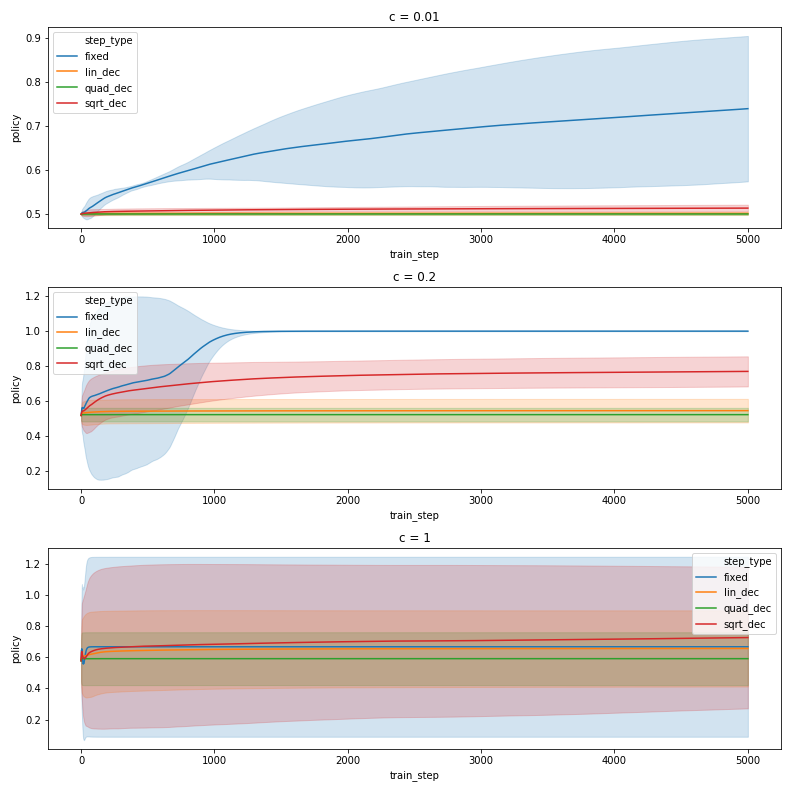
\includegraphics[width=\textwidth]
        {../img/policy_gradient_convergence_cs.png}}
        \caption{\label{fig:my-label} Influence of the step size}
      \end{figure}

\textbf{We find that, for small delta, only the fixed step size manages to get the right answer 100\% of the times. Using the other step sizes some seeds converge to the wrong policy, for a given initial c.} The issue here is that the learning rate decreases too fast to reach the optimal parameters, so we get stuck in the beginning. On the other hand, for larger learning rates, the policy jumps in the beginning and then gets stuck in a suboptimal level as well. \\

The optimal learning rate also depends on the parameters we are estimating. Since we are starting with small $\theta$, large learning rates send the parameters around by too much.

\subsection*{Question 2.3}

Task: Find the best step size and policy as function of $\Delta$. \\

\textbf{We observe faster convergence for big deltas.} This makes intuitive sense, since the "signal" from choosing the correct action is stronger for large deltas on average. For lower deltas we see that we sometimes don't even converge to the optimum.

   \begin{figure}[!htb]
        \center{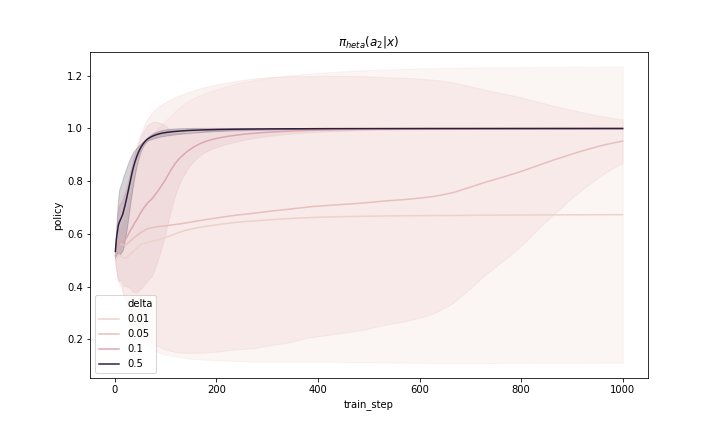
\includegraphics[width=\textwidth]
        {../img/policy_gradient_convergence_deltas.png}}
        \caption{\label{fig:my-label} Influence of delta}
      \end{figure}

\clearpage

\section*{Question 3}

Task: Performance of standard UCB and $\epsilon$-greedy algorithms

\subsection*{Question 3.1}

First we define the standard UCB algorithm for our bandit problem. As described in the question, at each iteration of the algorithm, we start by choosing an "arm" or action in this case by finding

$$I_{t}=\arg \max _{i \in\{1,2\}}\left(\widehat{\mu}_{t, i}+\sqrt{\frac{2 \ln t}{N_{t, i}}}\right)$$

we initialize the algorithm by forcing two trials of each action. After taking an action we store the resulting reward and update our mean estimator $\mu_{t,i}$.

The following plot shows the total reward for $T=10,000$ rounds as a function $\Delta$ of the environment:

\begin{figure}[H]
	\centering
	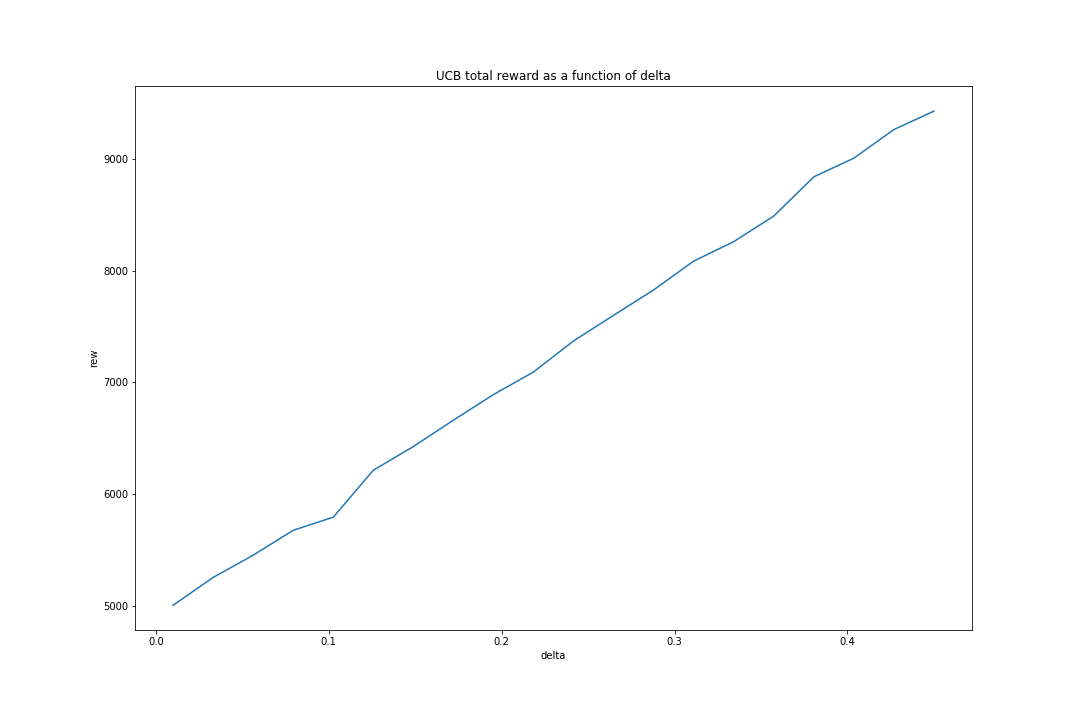
\includegraphics[scale = 0.4]{UCB_reward}
	\caption{}
\end{figure}

One can easily see that larger values of $\Delta$ lead to greater total rewards. The intuition behind this is that large $\Delta$ lead to a clear seperation between the expected rewards of each action. For very small $\Delta$, the expected rewards of each action are almost $\frac{1}{2}$. Unsurprisingly, the total reward for a $\Delta$ of 0 is 5000. Conversely, for a $\Delta$ of 0.5 the total reward is almost 10,000, but not quite. This is due to the fact that we still have to run a tiny amount of trials to get convergence of the estimated mean to the true value. After that we always pick the right action, which almost certainly results in a reward.

\subsection*{Question 3.2}

The $\epsilon$-greedy algorithm works in the following way:

For a given probability $\epsilon$, either choose a uniformly random action, or choose the action which has the maximum expected reward based on the previously recorded rewards. The value of $\epsilon$ drops in each step, resulting in a smaller and smaller chance of taking random actions. Consequently, the drop in $\epsilon$ can be seen as a switch from exploring the environment to exploiting it based on the reward history. $\epsilon$ in this case is set as $\epsilon = c/t$ where $c$ is a constant.

The following plot shows the total reward for a range of values of $c$ and $\Delta$.

\begin{figure}[H]
	\centering
	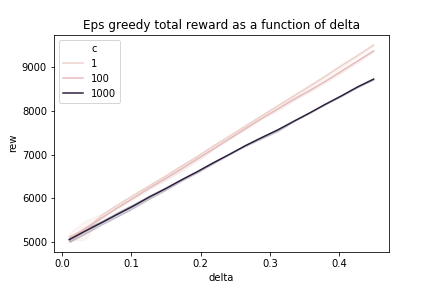
\includegraphics[scale = 0.6]{Eps_greedy_reward}
	\caption{}
\end{figure}

First we note that similarly to the UCB algorithm, larger values of $\Delta$ lead to higher total rewards. Additionally, for small $c$ and $\Delta$ all total rewards are similar. For greater $\Delta$, with smaller parameter $c$, the algorithm converges quicker to the optimal policy. This can be seen in the higher overall rewards. Again, the intuition is that for high $\Delta$ we don't need to explore the environment as in depth as before, so smaller $c$ will lead to a smaller amount of trials in which we randomly explore the environment.

\newpage

\subsection*{Question 3.3}

The last plot shows the combined results of all three algorithms for our small bandit problem with $T=10000$ for all runs.

\begin{figure}[h]
	\centering
	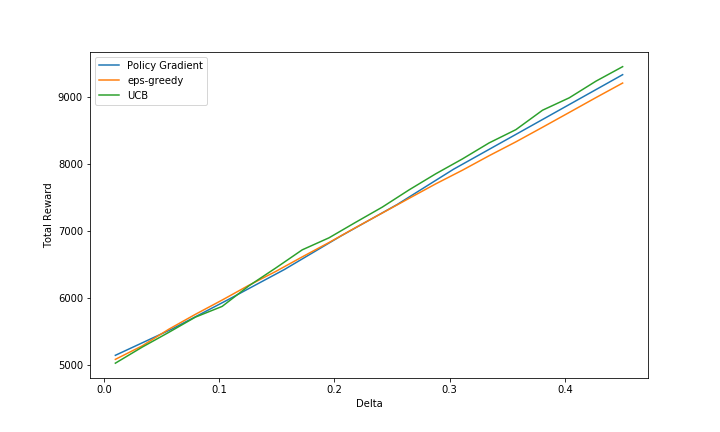
\includegraphics[scale = 0.6]{algorithms_comparison}
	\caption{}
\end{figure}

All algorithms have similar total rewards for a given $\Delta$ with UCB and Policy-Gradients being slightly better than $\epsilon$-greedy for larger $\Delta$. This is probably due to the fact that the problem at hand is a simple one, with only one state and two possible actions. In this case we don't loose too much if we use a "simple" policy like UCB, over the more complex policy gradient method. Further, finding the optimal learning rate for the policy gradient method is hard, whereas UCB is much simpler to implement and fine tune. 


\end{document}
